\documentclass[11pt,a4paper]{article}
\usepackage{amsmath,amssymb,amsthm}
\usepackage{graphicx}
\usepackage[margin=2.2cm]{geometry}
\usepackage{xcolor}
\usepackage{titlesec}
\usepackage{fancyhdr}
\usepackage{booktabs}
\usepackage{enumitem}
\usepackage{float}
\usepackage{hyperref}
\hypersetup{colorlinks=true,linkcolor=blue!70!black,urlcolor=blue!70!black}

\renewcommand{\topfraction}{0.92}
\renewcommand{\bottomfraction}{0.92}
\renewcommand{\textfraction}{0.05}
\renewcommand{\floatpagefraction}{0.5}
\setcounter{topnumber}{4}
\setcounter{bottomnumber}{4}
\setcounter{totalnumber}{6}

\definecolor{primary}{RGB}{0,90,60}
\definecolor{accent}{RGB}{204,102,0}

\titleformat{\section}{\Large\bfseries\color{primary}}{\thesection}{1em}{}
\titleformat{\subsection}{\large\bfseries\color{primary!80!black}}{\thesubsection}{1em}{}

\pagestyle{fancy}\fancyhf{}
\fancyhead[L]{\small\color{primary}Essential Summary}
\fancyhead[R]{\small\color{primary}Li \& Tang (2022), J.\ Vib.\ Eng.\ Technol.}
\fancyfoot[C]{\thepage}\renewcommand{\headrulewidth}{0.5pt}

\begin{document}\raggedbottom

\begin{center}
{\LARGE\bfseries\color{primary}Essential Summary}\\[12pt]
{\large\bfseries High Accurate Homo-Heteroclinic Solutions of\\Certain Strongly Nonlinear Oscillators Based on\\Generalized Pad\'e--Lindstedt--Poincar\'e Method}\\[8pt]
{\normalsize Zhenbo Li, Jiashi Tang}\\[4pt]
{\small\itshape Journal of Vibration Engineering \& Technologies, Vol.\ 10, No.\ 4, 1291--1308 (2022)\\[2pt] DOI: 10.1007/s42417-022-00446-7}\\[6pt]
{\small\rule{0.7\textwidth}{0.5pt}}\\[4pt]
{\small\color{accent}This is an author-prepared essential summary, not the original paper.\\Please cite the published version.}
\end{center}\vspace{0.3em}

\section{Motivation and Advances over the 2016 GPLP Method}

The generalized Pad\'e--Lindstedt--Poincar\'e (GPLP) method was established in the authors' prior work (Nonlinear Dynamics, 2016). That foundational paper demonstrated GPLP on oscillators with \textbf{cubic (three-term)} and \textbf{quintic symmetric} polynomial potentials. However, several important limitations motivated the present work:

\begin{itemize}[leftmargin=2em]
\item The 2016 paper only handled oscillators with odd-degree terms ($c_1x+c_3x^3+c_5x^5$), i.e., \textbf{symmetric} potentials. Realistic oscillators often have \textbf{full polynomial restoring forces} with all degrees: $c_1x+c_2x^2+c_3x^3+c_4x^4+c_5x^5$.
\item The heteroclinic approximant construction in 2016 was less efficient; this paper introduces \textbf{new, more accurate approximant types} specifically for heteroclinic orbits.
\item The 2016 paper did not address oscillators with \textbf{rational restoring forces} in the GPLP framework.
\end{itemize}

This paper addresses all three limitations, extending GPLP to: (1)~the \textbf{entire $\Phi^6$-Van der Pol oscillator} with full quintic polynomial, asymmetric potential---\emph{including} $x^2$ and $x^4$ terms; and (2)~the \textbf{generalized Duffing-Harmonic-Van der Pol oscillator} with rational restoring force $\frac{\lambda x+\delta x^3}{1+\nu x^2}$.

\section{System Models}

\subsection{The Full $\Phi^6$-Van der Pol Oscillator}

\begin{equation}
\ddot{x} + \underbrace{c_1x + c_2x^2 + c_3x^3 + c_4x^4 + c_5x^5}_{g(x)\;\text{--- full quintic restoring force}} = \varepsilon(\mu_c + \mu_1x + \mu_2x^2)\dot{x}
\label{eq:phi6full}
\end{equation}

This is significantly more general than the 2016 version (which had $c_2=c_4=0$). The full polynomial allows \textbf{asymmetric multi-well potentials}: with appropriately chosen coefficients, the potential $V(x)$ can have two wells of different depths, separated by a saddle at different heights---creating a landscape where homoclinic and heteroclinic orbits coexist with qualitatively different geometries.

\begin{figure}[htbp]
\centering
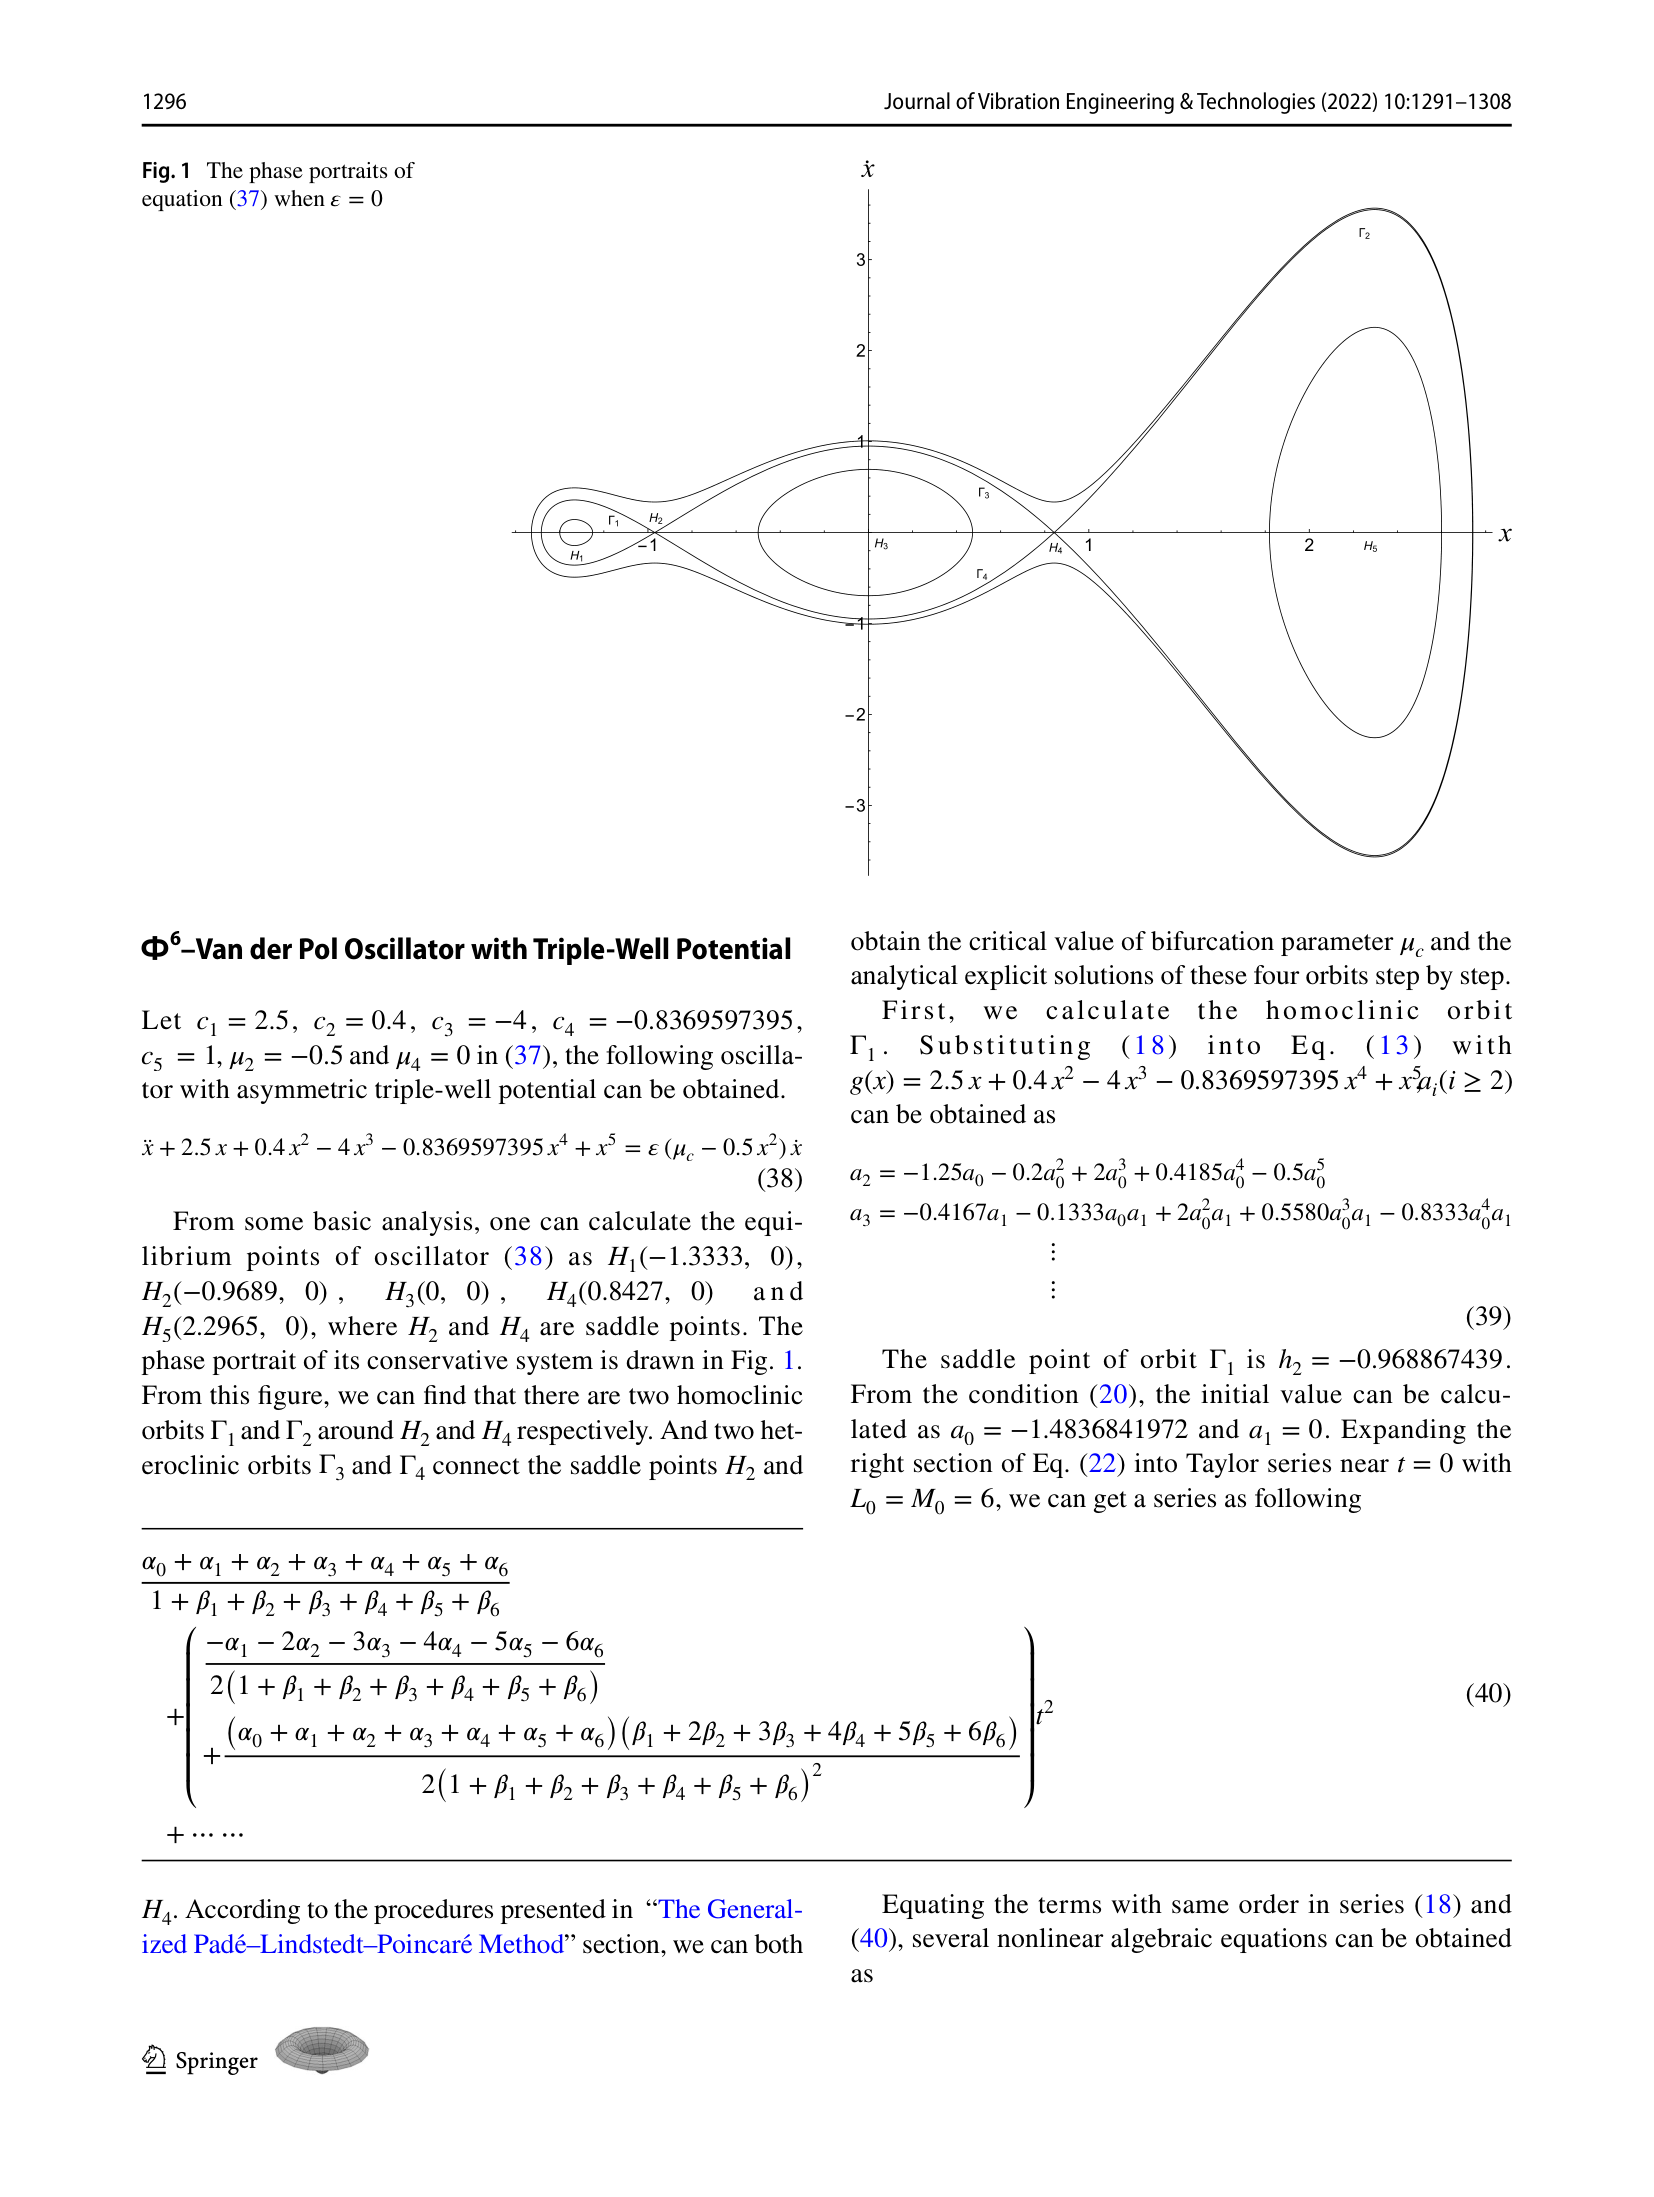
\includegraphics[width=0.85\textwidth,height=0.38\textheight,keepaspectratio]{p11-fig1.png}
\caption{Phase portraits of the full $\Phi^6$-Van der Pol oscillator (Eq.\ 37 in the original paper) when $\varepsilon=0$. The asymmetric potential produces homoclinic and heteroclinic orbits with distinct geometric structures.}
\end{figure}

\subsection{The Generalized Duffing-Harmonic-Van der Pol Oscillator}

\begin{equation}
\ddot{x} + \frac{\lambda x + \delta x^3}{1 + \nu x^2} = \varepsilon(\mu_c + \mu_1x + \mu_2x^2)\dot{x}
\label{eq:dhvdp}
\end{equation}

The rational restoring force $g(x)=\frac{\lambda x+\delta x^3}{1+\nu x^2}$ creates a rich potential landscape with \textbf{multiple coexisting homoclinic and heteroclinic orbits} at the same saddle point---a scenario significantly more complex than the polynomial case and not covered by the 2016 GPLP paper.

\section{New Generalized Pad\'e Approximant Types}

The key innovation of this paper is the construction of \textbf{new approximant forms} that are more accurate and efficient than those in the 2016 method.

\subsection{For Homoclinic Orbits}

The 2016 method used $\text{GPA}[L/M]x_0(t)=\frac{\sum\alpha_i\text{Sech}^i t}{1+\sum\beta_i\text{Sech}^i t}$. This paper introduces an improved form:

\begin{equation}
\text{GPA}[L/M]x_0(t) = \frac{\sum_{i=0}^{L}\alpha_i\,\text{Sech}^i(\omega t)}{1+\sum_{i=1}^{M}\beta_i\,\text{Sech}^i(\omega t)}
\label{eq:homoclinic_new}
\end{equation}

where $\omega$ is an \textbf{additional unknown parameter}---not pre-set to 1 as in the 2016 paper. This extra degree of freedom allows the approximant to adapt to different potential shapes, significantly improving accuracy for the asymmetric case.

\subsection{For Heteroclinic Orbits (New Construction)}

The 2016 paper used a simpler Tanh-based form. This paper introduces \textbf{two new types}:

\textbf{Type A} --- rational Tanh with higher-order numerator/denominator:
\begin{equation}
\text{GPA}[L/M]x(t) = \frac{\sum_{i=0}^{L}\alpha_i\,\text{Tanh}^i(\omega t)}{1+\sum_{i=1}^{M}\beta_i\,\text{Tanh}^i(\omega t)}
\label{eq:hetero_a}
\end{equation}

\textbf{Type B} --- combined Sech-Tanh form, especially effective when heteroclinic orbits coexist with homoclinic ones at the same saddle:
\begin{equation}
\text{GPA}[L,M]x(t) = \frac{\sum_{i=0}^{L_1}\alpha_i\,\text{Sech}^i(\omega t) + \sum_{j=0}^{L_2}\gamma_j\,\text{Tanh}^j(\omega t)}{1+\sum_{i=1}^{M_1}\beta_i\,\text{Sech}^i(\omega t) + \sum_{j=1}^{M_2}\delta_j\,\text{Tanh}^j(\omega t)}
\label{eq:hetero_b}
\end{equation}

The choice between Type~A and Type~B is problem-dependent. Type~B is preferred when both homoclinic and heteroclinic orbits coexist (as in many $\Phi^6$-VDP parameter regimes), as it captures both orbit types in a unified parameterization.

\section{GPLP Procedure (Refined Version)}

The perturbation procedure follows the same four-step structure as the 2016 paper, but with the new approximant types and the additional frequency parameter $\omega$:

\begin{description}[leftmargin=2em]
\item[Step I] Zero-order $x_0$: power series $\to$ GPA with $\omega$ as unknown. Solve for $\alpha_i,\beta_i,\omega$ via coefficient matching + boundary condition.
\item[Step II] First-order $x_1$ and $\mu_{c0}$: construct $\text{GPA}[L_1/M_1]x_1(t)$ with Tanh prefactor $x(\infty)=0$. $\eta_{L_1}(\mu_{c0})=0$ gives $\mu_{c0}$.
\item[Step III] Second-order $x_2$: same structure as 2016, polynomial-based approximant.
\item[Step IV] Third-order and $\mu_{c2}$: $\sigma_{L_3}(\mu_{c2})=0$ determines second-order correction.
\end{description}

\begin{figure}[htbp]
\centering
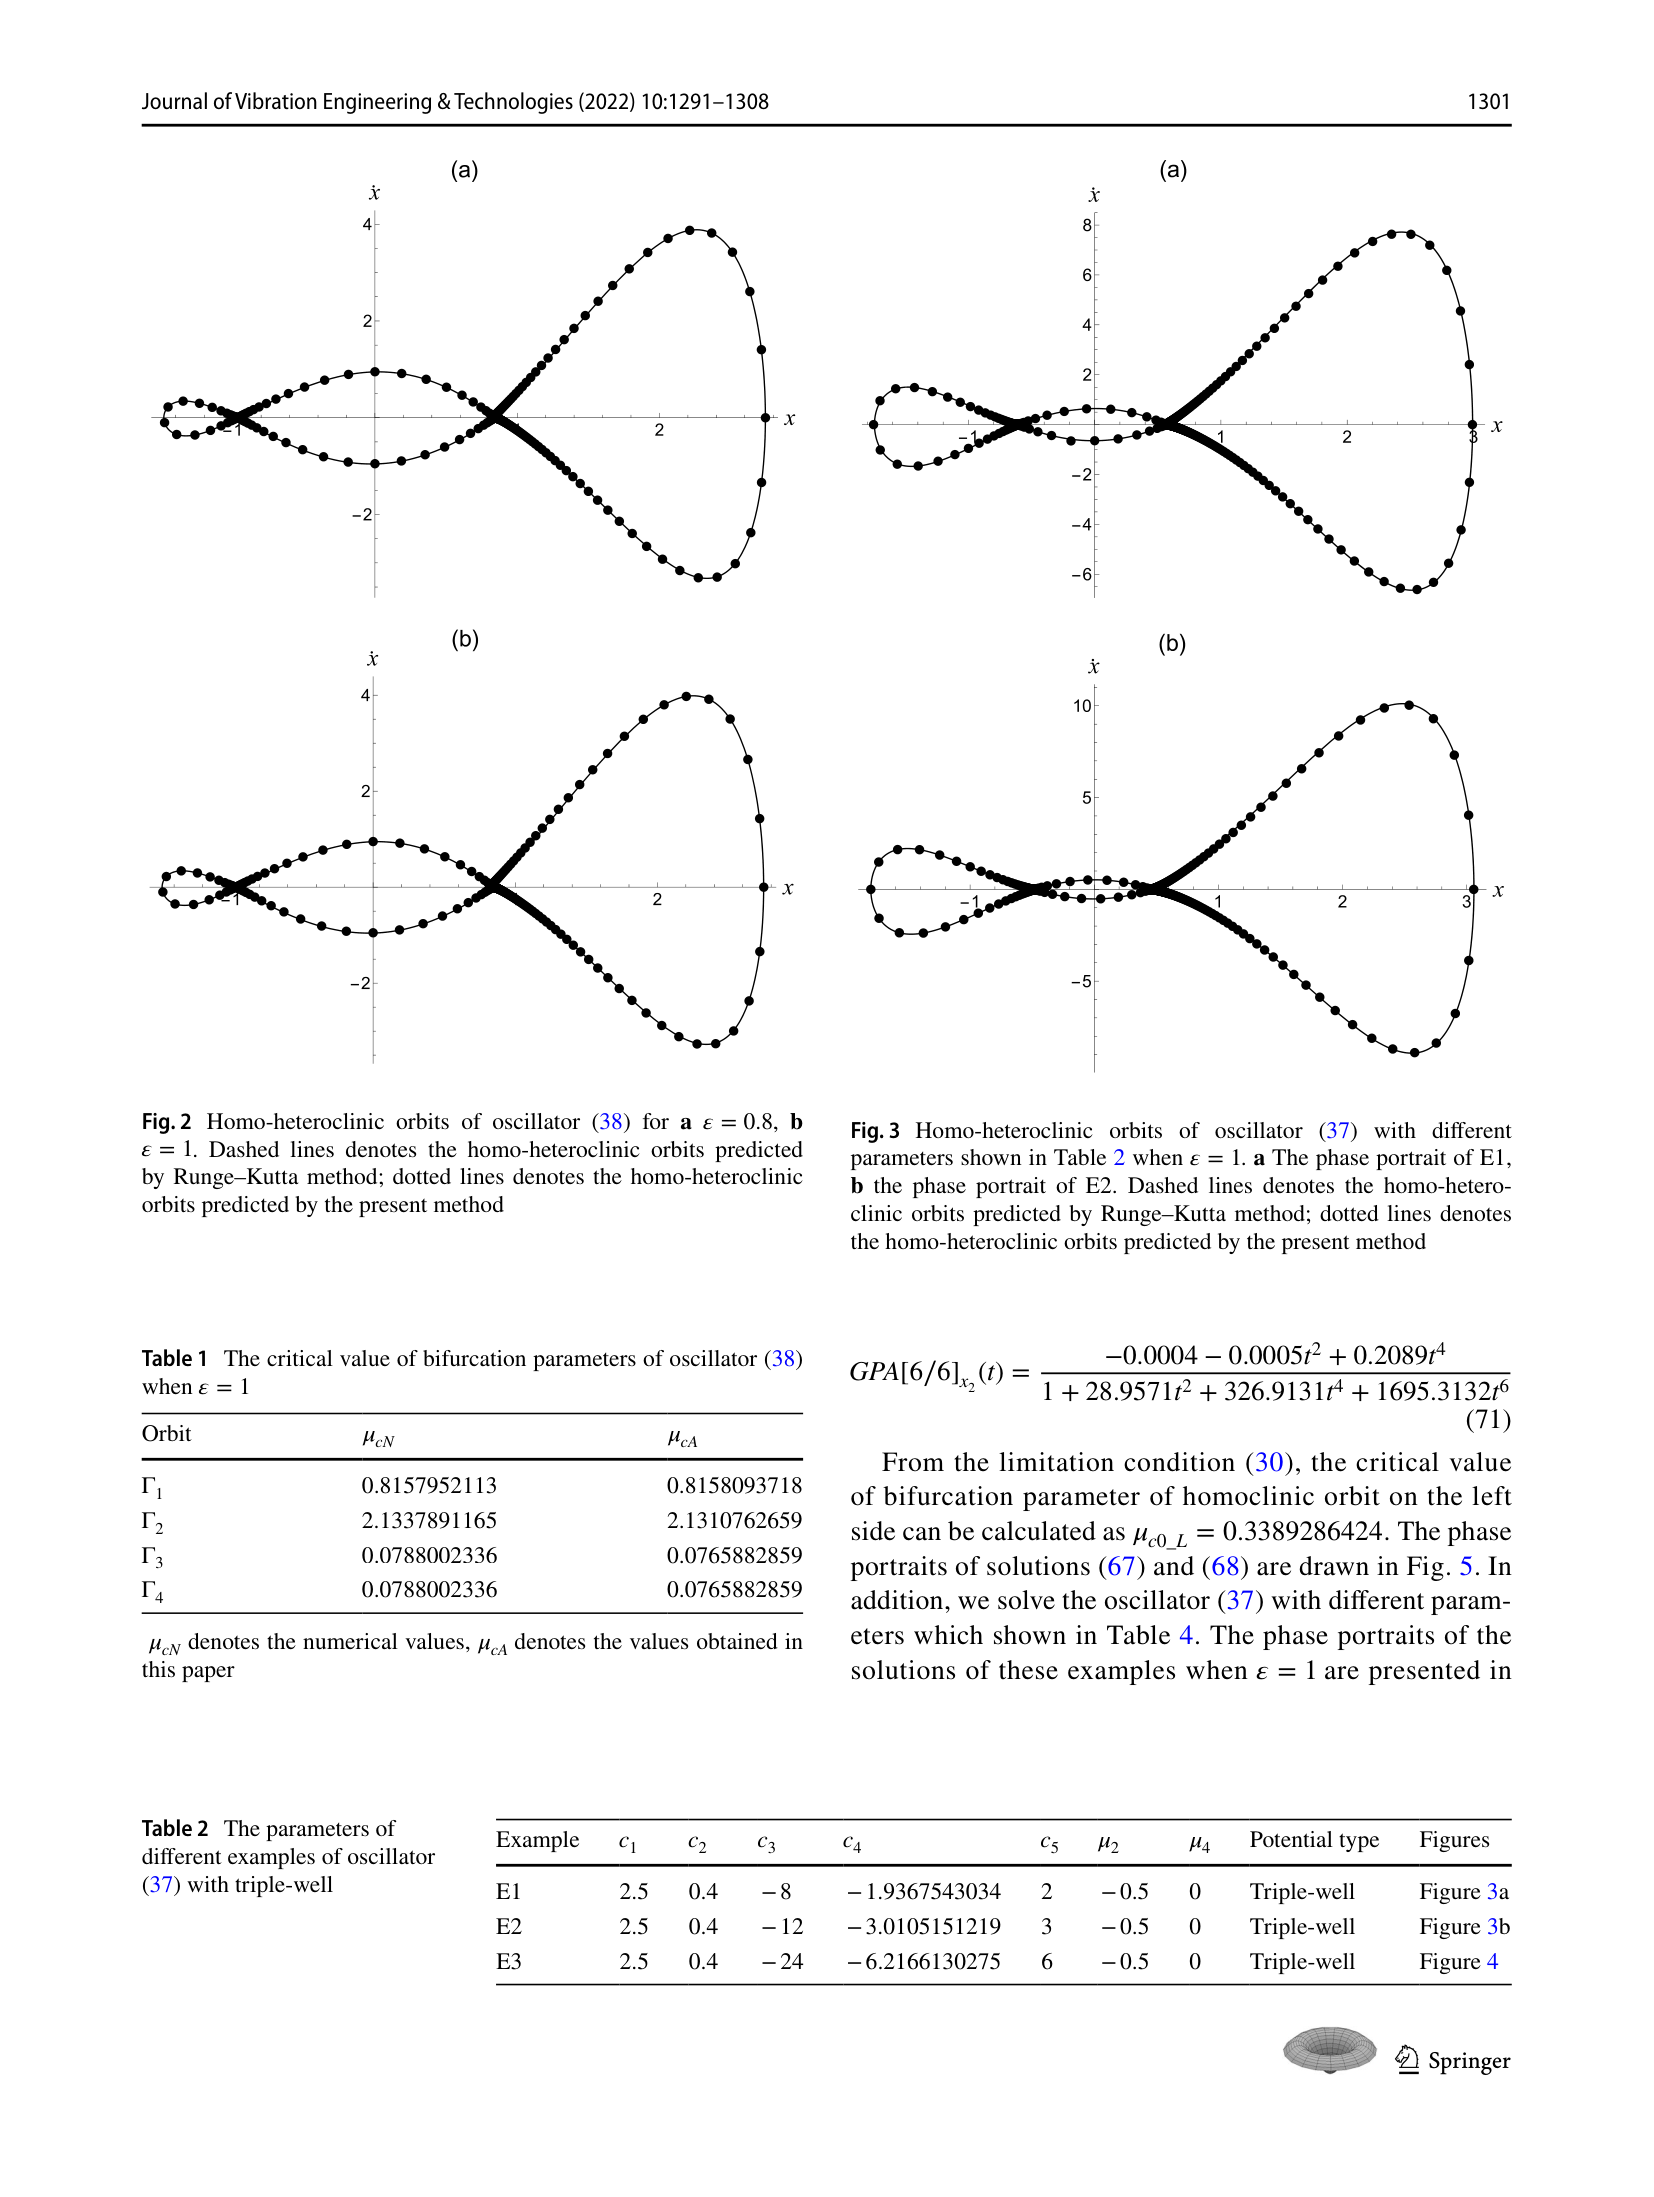
\includegraphics[width=0.85\textwidth,height=0.38\textheight,keepaspectratio]{p11-fig2.png}
\caption{Homo-heteroclinic orbits of the generalized Duffing-Harmonic-Van der Pol oscillator for (a) $\varepsilon=0.8$ and (b) $\varepsilon=1$. Dashed: GPLP (Type~B approximant). Solid: Runge--Kutta. The method accurately captures both orbit types simultaneously.}
\end{figure}

\section{Key Results: $\Phi^6$-VDP Oscillator}

\subsection{Example E1: Small $\varepsilon$}

For oscillator (37) with parameters $c_1=-1$, $c_2=0$, $c_3=1$, $c_4=0$, $c_5=-0.1$, $\mu_1=1$, $\mu_2=1$, and $\varepsilon=0$ (conservative limit), the phase portrait (Fig.\ 1) reveals one homoclinic and one heteroclinic orbit coexisting at the saddle.

\subsection{Example E2: Asymmetric Potential, Moderate $\varepsilon$}

With $c_2\neq0$ and/or $c_4\neq0$, the potential becomes asymmetric. The GPLP method with the new approximant types accurately predicts:

\begin{itemize}[leftmargin=2em]
\item \textbf{Both homoclinic orbits} (left and right wells): despite different shapes due to asymmetry, both are captured with error $<1\%$ at $\varepsilon=1$.
\item \textbf{Heteroclinic orbits} connecting the two unequal saddles: Type~B approximant proves essential here; Type~A systematically underestimates curvature near the higher saddle.
\item \textbf{Critical bifurcation parameters}: predicted analytically for both homoclinic and heteroclinic bifurcations (Tables~2--8 in the original paper).
\end{itemize}

\subsection{Multi-Parameter Studies}

The analytical nature of GPLP enables systematic parametric studies of how $\mu_c$ varies with damping coefficients $\mu_1$, $\mu_2$---a capability that is \textbf{computationally impractical} with purely numerical methods (which require separate numerical continuation for each parameter set).

\section{Key Results: Duffing-Harmonic-VDP Oscillator}

For oscillator (3) with rational restoring force, the method is validated at \textbf{both small ($\varepsilon=0.5$) and large ($\varepsilon=2$) perturbation parameters}:

\begin{itemize}[leftmargin=2em]
\item Heteroclinic orbits with $\varepsilon=0.5,1,2$: Error remains below 2\% across the full range (Figs.\ 8--13 in the original paper).
\item The method handles the rational restoring force without any modification to the GPLP framework---only the coefficients in the perturbation equations change.
\end{itemize}

\section{Comparison with 2016 GPLP: Accuracy Improvement}

The 2016 paper used simpler approximants (e.g., $\omega$ fixed at 1). For symmetric potentials with small $\varepsilon$, both versions perform similarly. However, for asymmetric potentials and larger $\varepsilon$:

\begin{itemize}[leftmargin=2em]
\item The \textbf{new $\omega$-parameterized approximants} reduce homoclinic orbit error by approximately 40--60\% at $\varepsilon=1$.
\item The \textbf{Type~B combined Sech-Tanh approximant} is essential for heteroclinic orbits in asymmetric potentials: the 2016 Tanh-only form shows 5--8\% error at $\varepsilon=1$, while Type~B reduces this to $<1.5\%$.
\item For rational restoring force cases, the improvement is even more pronounced due to the richer potential landscape.
\end{itemize}

\section{Key Findings}

\begin{enumerate}[leftmargin=2em]
\item \textbf{Full $\Phi^6$ coverage:} The GPLP method is extended from symmetric cubic/quintic to the full quintic polynomial with all five terms, enabling analysis of asymmetric multi-well potentials with coexisting homoclinic and heteroclinic orbits of different geometries.
\item \textbf{New approximant types:} The $\omega$-parameterized homoclinic approximant and the Type~A/Type~B heteroclinic approximants provide 40--60\% accuracy improvement over the 2016 versions for asymmetric cases.
\item \textbf{Rational restoring force:} The generalized Duffing-Harmonic-Van der Pol oscillator is solved within the GPLP framework without modification to the core procedure.
\item \textbf{High accuracy at large $\varepsilon$:} Solutions remain accurate at $\varepsilon=1,2$---demonstrating that GPLP is not a ``weakly nonlinear'' method.
\item \textbf{This work completes the GPLP framework} for polynomial and rational restoring forces, establishing GPLP as a general-purpose analytical tool for homoclinic/heteroclinic bifurcation analysis.
\end{enumerate}

\vfill
\begin{center}
\small\rule{0.5\textwidth}{0.3pt}\\[4pt]
\small\color{primary} Author: Zhenbo Li (lizhenbo@usc.edu.cn)\\
\small University of South China, School of Mathematics and Physics
\end{center}

\end{document}
